% Template:     Informe LaTeX
% Documento:    Archivo de ejemplo
% Versión:      8.1.7 (24/07/2022)
% Codificación: UTF-8
%
% Autor: Pablo Pizarro R.
%        pablo@ppizarror.com
%
% Manual template: [https://latex.ppizarror.com/informe]
% Licencia MIT:    [https://opensource.org/licenses/MIT]

\section{Introducción}

\lipsum[2-4]

\section{Configuración de una instancia EC2}
\subsection{Inicio de sesión en AWS}

\begin{figure}[h]
	\centering
	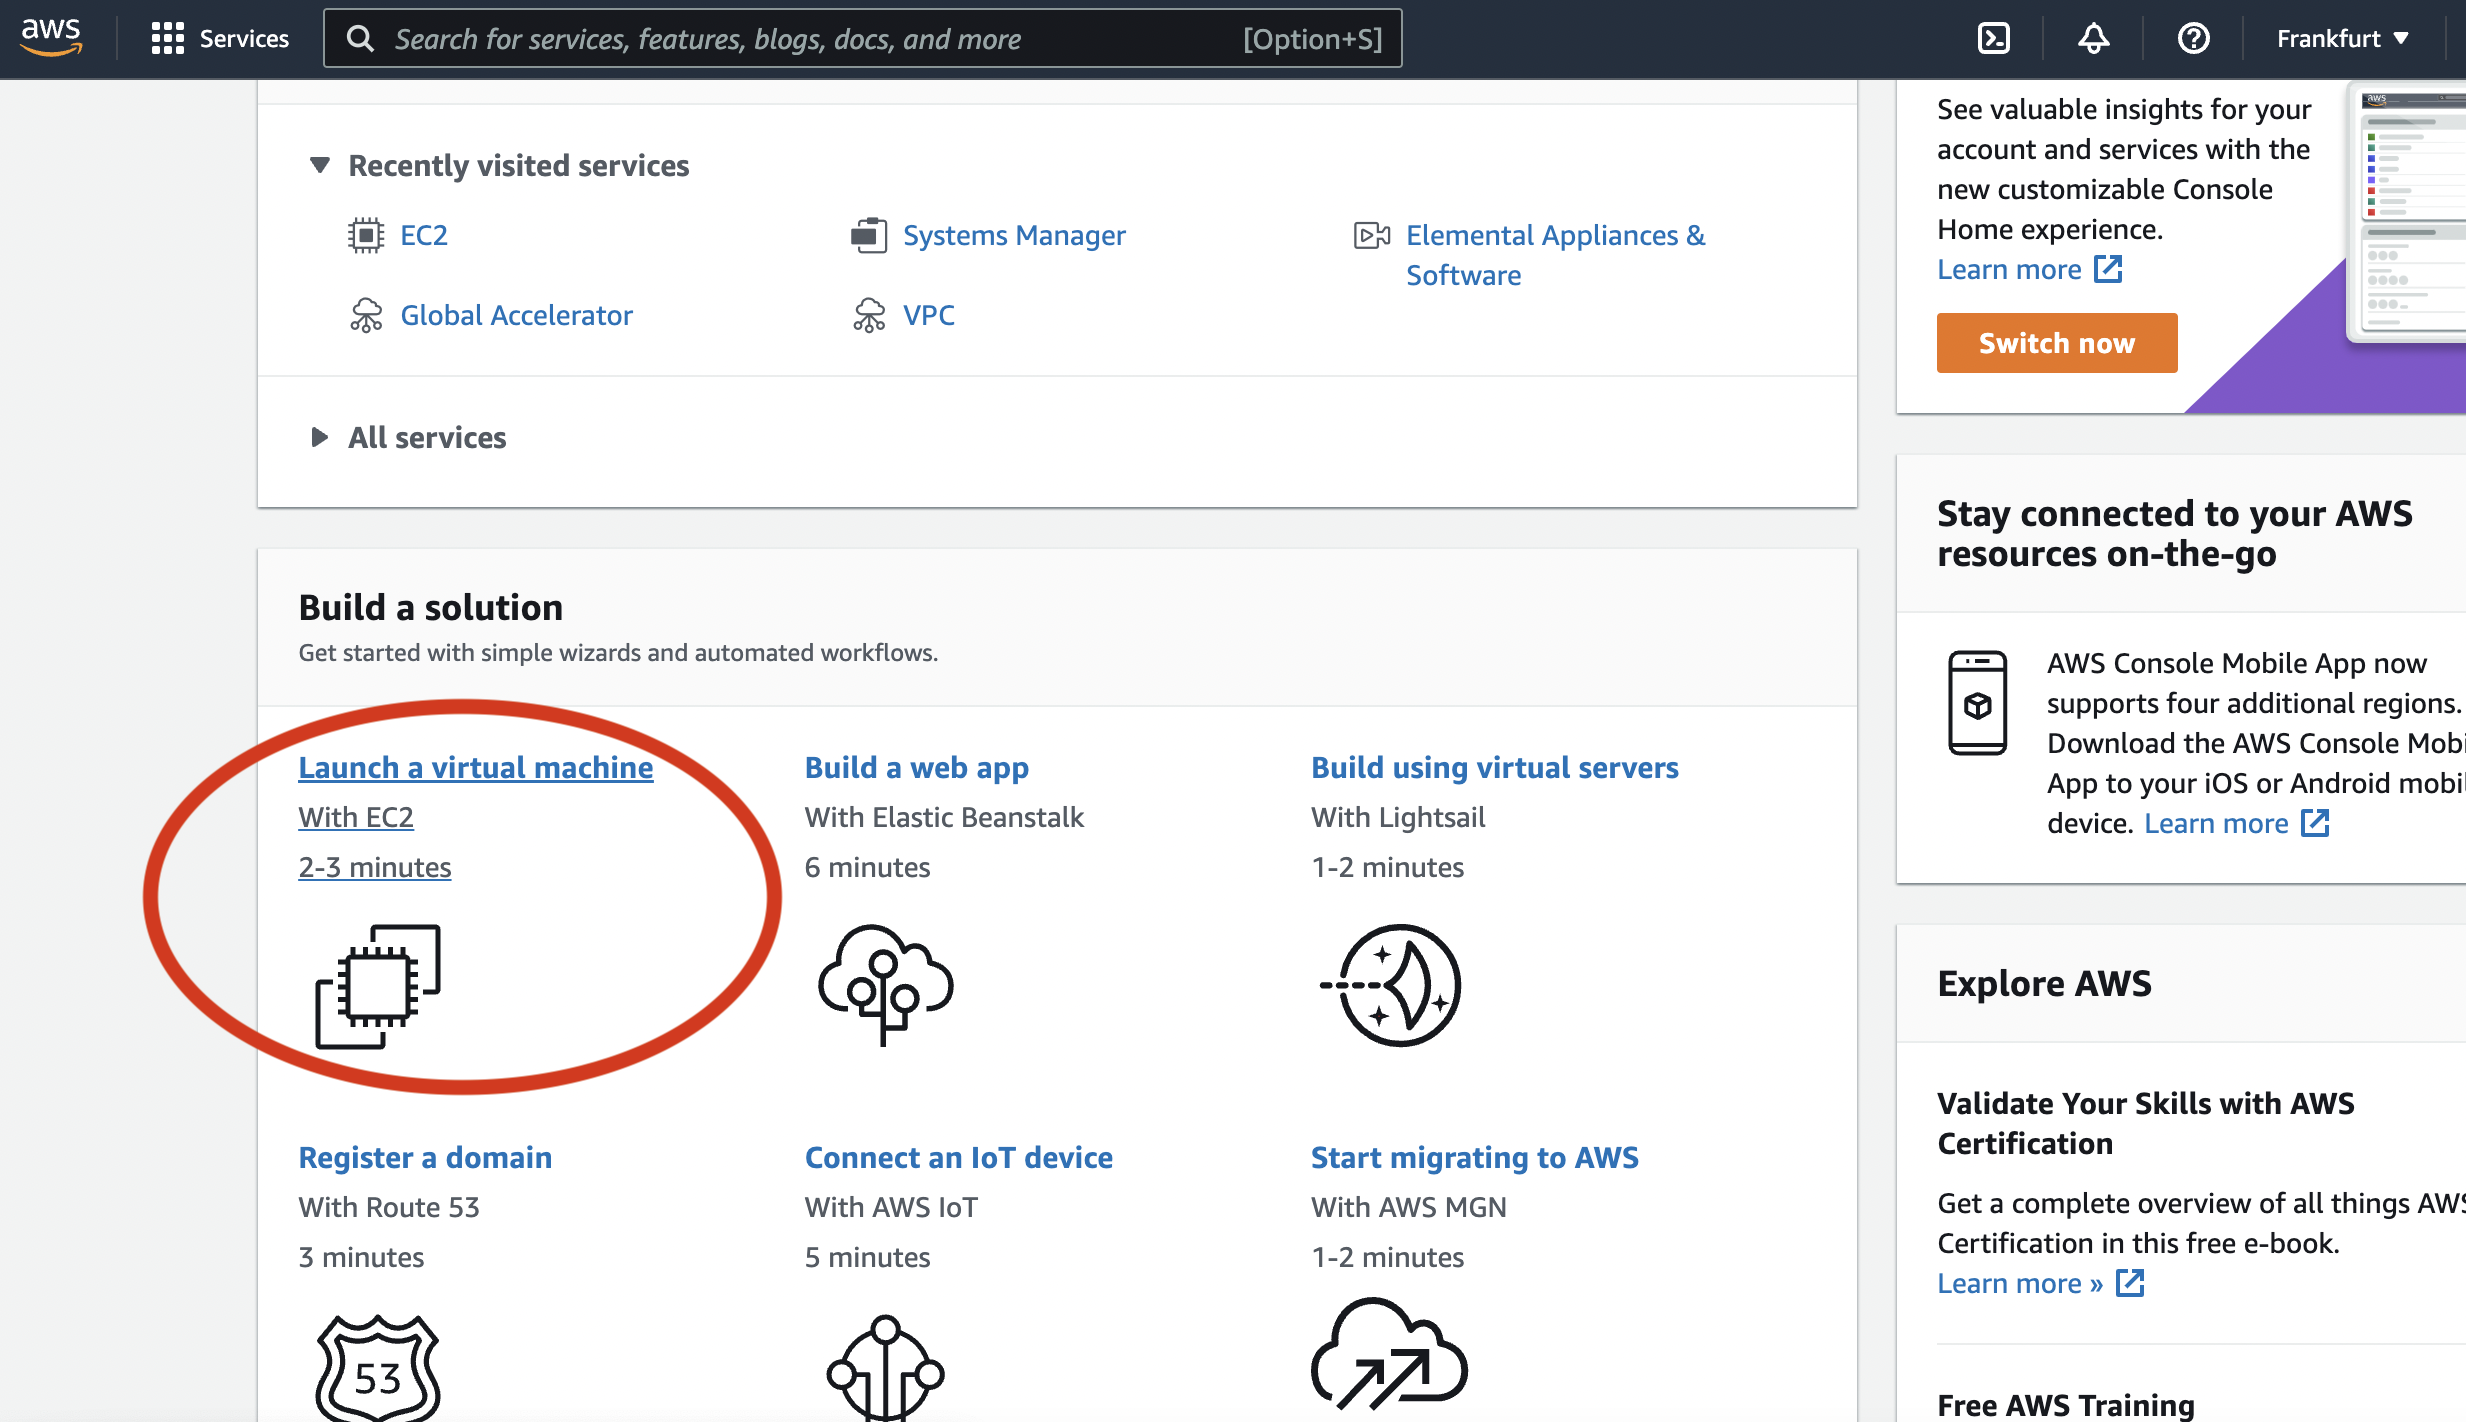
\includegraphics[scale=.3] {img/ejemplo}
	\caption{Sistema de recomendación por asociación de productos, Fuente: \scite{singh2019analysis}}
	\label{fig:5}	
\end{figure} 

\lipsum[2-4]

\subsection{Selección de imagen AMI}
\lipsum[2-4]

\subsection{Elección del tipo de instancia}
\lipsum[2-4]

\subsection{Configuración de IP público}
\lipsum[2-4]

\subsection{Configuración de espacio de almacenamiento}
\lipsum[2-4]

\subsection{Configuración del Grupo de Seguridad}
\lipsum[2-4]

\subsection{creación de clave privada}
\lipsum[2-4]

\subsection{Iniciar instancia}
\lipsum[2-4]


\subsection{Asignación de IP estática a la instancia}
\lipsum[2-4]

\subsection{Asociación de IP estática a la instancia}
\lipsum[2-4]

Conexión segura por SSH


Actualización de paquetes


Cambio de nombre al hostname

Instalación de OpenJDK


Descarga e instalación de Hadoop


Descompresión e instalación del instalador

cambiando y moviendo el paquete

Configuración del environment

Conexión segura por SSH

 

\subsection{Configuración de Hadoop}
\lipsum[2-4]


-
-
-

\subsection{Inicio de Cluster de Hadoop}
\lipsum[2-4]

-
-
-





\section{Ejemplo de Aplicación WordCount con Mapreduce}
\lipsum[2-4]

- Código Fuente

- Crear un archivo de entrada


- Crear un directorio en HDFS y copiar archivos de Local a HDFS


- Ejecución de MapReduce

- Salida



\section{Conclusiones}
\lipsum[2-2]
% ------------------------------------------------------------------------------
% REFERENCIAS, revisar configuración \stylecitereferences
% ------------------------------------------------------------------------------
\clearpage
\bibliography{library} 